\documentclass[11pt,a4paper]{ivoa}
\input tthdefs

\newcommand{\xtype}[1]{\texttt{#1}}

\usepackage{listings}
\lstloadlanguages{XML,SQL}
\lstset{flexiblecolumns=true,basicstyle=\ttfamily}
\usepackage[utf8]{inputenc}
\usepackage{todonotes}
\usepackage{textcomp}
\usepackage{float}
\usepackage{lscape}
\usepackage{longtable}
\hyphenation{imagemosaic}

\marginparwidth=4cm

\title{IVOA Obscore Extension for Radio data}

\ivoagroup{Data Model Working Group}

\author{Fran\c cois Bonnarel}
\author{Mireille Louys}
\author{Baptiste Cecconi}
\author{Vincenzo Galluzzi}
\author{Yan Grange}
\author{Mark Kettenis}
\author{Mark Lacy}
\author{Alan Loh}
\author{Mattia Mancini}
\author{Peter Teuben}
\author{Alessandra Zanichelli}




\editor{Fran\c cois Bonnarel, Mark Kettenis , Mireille Louys}

\previousversion{}




%definition of table names 
%\def\radioexttable {ivoa.obscore-radio-ext} % explicit 
\def\radioexttable {ivoa.obsradio} % not explicitely related to Obscore 
\def\radioexttable {ivoa.obscore-radio} 
%definition of standard id for  utypes content 
%\def\obsradioSTDID {ivo://ivoa.net/std/obscore-radio-ext#table-1.0}

\begin{document}

\begin{abstract}
This is a proposed extension to the ObsCore specification for data description, discovery and selection of radio data.
\end{abstract}

\section*{Acknowledgments}

The authors would like to thank all the participants in DM-WG and Radioastronomy-IG discussions
for their ideas, critical reviews, and contributions to this document.
We acknowledge also the support of  ESCAPE (European Science Cluster of Astronomy
and Particle Physics ESFRI Research Infrastructures) funded by the EU Horizon
2020 research and innovation program (Grant Agreement no 824064).
% are there other grants from partners to mention here?

\section{Introduction}


ObsCore specification \citep{2017ivoa.spec.0509L} defines both a minimal datamodel to describe datasets
and a table consistent with the model which can be served by TAP services. It has been successful
to define a lot of data discovery services in astronomy.

The emergence  of  the Radioastronomy Interest Group in the IVOA in April 2020 confirmed the strong
interest of the radio astronomy community to distribute their data in the VO. Many teams now
distribute their data using VO standards\footnote{https://ivoa.net/documents/Notes/RadioVOImp/index.html}.
While reduced radio data products, such as images or spectral cubes,%(and single dish data - {\it is that true ?} )
are mostly covered by the ObsCore model, the lower level observational data
(interferometric visibilities, single dish data in SDFITS, filterbank or whatever other specific formats) require additional description parameters.
For interferometry, this need  was already exposed
in 2010 by Anita Richards in a IVOA Note  "Radio interferometry data in the VO" 
\footnote{https://wiki.ivoa.net/internal/IVOA/SiaInterface/Anita-InterferometryVO.pdf} which captures precisely the requirements in the radio community.
 
 Various discovery use cases have been collected in the radio community and gathered in the \ref{ADQLusecases} appendix.
  The current specification suggests addition of new features in the ObsCore metadata profile to fill the gap.
% Mireille an attempt to widen the scope ??
With the expansion of large radio astronomy projects such as LOFAR, NenuFAR, the future SKA, ngVLA, etc...
and the emergence of interesting research topics matching data in all electromagnetic regimes, the
Virtual Observatory framework can facilitate a wider access to radio data for experts and
non-specialists radio astronomers in order to support collaborations in multi-wavelength,
multi-messenger astronomy.

%mireille:
% the needs for today as explored in recent meetings in Escape framework can also be summarized here
% add a short paragraph here
%Although the interferometry data are nowadays dominant in radio field, similar issues occur for
%optical interferometry data. The extension we are defining here is valid for both domains.
\begin{figure}
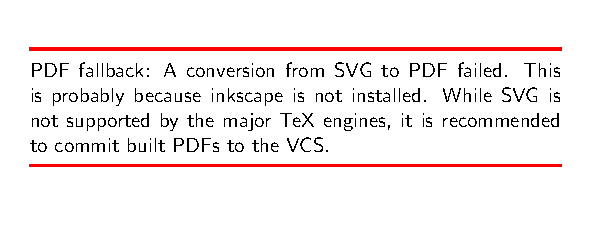
\includegraphics[width=0.9\textwidth]{role_diagram.pdf}
\label{fig:architecture}
\end{figure}
% Mireille : it seems this is not the good diagram but the one of SIA
% change architexture diag

%The role of this Visibility ObsCore extension in the IVOA is very close to ObsCore itself. It's only a fine grain improvement of this specification. 
% Mireille's  suggestion
This Radio ObsCore extension in the IVOA, relies  on ObsCore itself and expands it
to allow data providers to describe their radio data further the  ObsTAP framework.
Its goal is to clarify how  ObsCore metadata  can be used in the  radio context and to add new specific features to the existing ObsCore metadata.


\section{Radio data specifities from the Data Discovery point of view}
\label{sec:specificities}


On the lower end of the radio spectrum, radio astronomers generally make use of
frequencies for designating the spectral ranges of their observation. The standard
ObsCore attributes \emph{em\_min, em\_max} are expressed in wavelength and are not really convenient.
That's why we should also provide a mechanism for  translation into frequencies .But this should not be done by duplicating the same information in two different attributes. 

Receivers with a (ultra)wide bandwidth, up to tens of GHz, are
nowadays commonly used for both interferometric and Single Dish (herefater SD) radio observations.
Given that the spatial field of view and resolution linearly depend on wavelength, these quantities may significantly vary across the observed bandwidth in a radio observation.
Generally only a representative value (for instance the
%median
receiver nominal frequency) for these two parameters can be given. It is
noticeable that this is the case for any measuring system allowing a large interval of
$\lambda/D$ (where $\lambda$ and $D$ are the wavelength and the measuring system
aperture scale).
 
Similarly, the resolution power quantity, commonly provided to describe optical spectroscopic data, is generally not used in the radio domain.
Instead one could introduce a new ObsCore element for the absolute spectral resolution, in frequency unit, for which a representative value for each observation can be given.

Modern radio instrumentation offers the possibility of several  spectral windows within the same observation with significant separation or different resolutions.
Such observations may be represented at the highest granularity as  a set of combined data sets represented by several entries in an ObsCore table. However it's up to data provider to decide which level of granularity is best adapted in order to optimize data discoverability and ease data access, depending on the scientific content of the observation.
%(see Sect. \ref{subsec:sd} for an example).



\subsection{Single dish data}\label{subsec:sd}

Single Dish (SD) observations can be done with different types of receiving systems. Typical frontends are mono-feed, multi-feed and phased array feed (PAF), the last two suitable to efficiently span wider parts of the sky.
Data can be acquired by various backend systems providing either the total intensity (integrated over the whole available bandwidth) or the spectroscopic/spectropolarimetric intensity (acquired in each spectral channel/sample).
Data are saved as raw counts resulting from the digitization of the voltage signal measured by the receiving system.
Commonly-used SD data formats are registered FITS standard conventions (FITS, SDFITS and MBFITS) or unregistered conventions like the standard FITS-based format delivered by the INAF radio telescopes.

The combination of telescope, frontend and backend permits the realization of various observing strategies characterized by specific spatial and/or spectral patterns.
Typical SD observing strategies are: \texttt{on-source}, \texttt{frequency switching}, \texttt{on-off} observations, \texttt{raster} or \texttt{on-the-fly} (OTF) mapping, \texttt{on-the-fly-cross-scan}, \texttt{skydip} calibrations (see Fig~\ref{fig:SD}). For each spatial position in the observation, SD data gather emission for any of the spectral samples in the given frequency band and polarization.
If multi-feed/PAFs are used, a set of spatial positions are simultaneously measured. Scan modes should be described in ObsCore in order to allow astronomers to better understand the structure of the data which will be retrieved.

Spatial resolution in the SD case is intended as the beam size. This holds true for any type of receivers, since also for multi-feed/PAF ones the spatial resolution is ruled by the size of the individual beam.

Contrary to what usually happens for  interferometric observations, for some radio telescopes a SD observation (scan) contains only one scientific target (for example INAF ones). In any case, each target in an observation is listed as a separate entry in an ObsCore table sharing the same \emph{obs\_id}.

Complex frequency setups are possible in the same observation, as already mentioned in Sect. \ref{sec:specificities}.

The ObsCore parameter \emph{t\_resolution}, defined as the minimal interpretable interval between two points along the
time axis (being it an average or representative value), has a limited application for SD data except for \texttt{on-source} tracking observations like those for pulsar/FRB studies.
Typically, time is not an independent variable in SD measurements and it can be saved together with spatial/spectral/intensity
information as a timestamp associated to each data sample. 
A more comprehensive discussion on ObsCore parameters for time-domain data is given in the Pulsar
and FRB Radio Data Discovery and Access IVOA Note\footnote{\url{https://wiki.ivoa.net/internal/IVOA/RadioastronomyInterestGroupFifthVirtualMeeting/PulsarRadioDataAccess.pdf}}.
%Even in the case of on-source tracking, time information in SD data is not intended for time domain studies.


\begin{figure}[H]
\centering
\includegraphics[width=0.9\textwidth]{SingleDish.png}
\caption{Single Dish Observation scan modes}
\label{fig:SD}
\end{figure}


\subsection{Visibility data }
\label{sec:visibility}

Visibility data are sets of complex numbers corresponding to the amplitude and phase
of correlation coefficients measured between pair of antennas (i.e., a baseline), at
a given time, a given wavelength or polarisation. The visibility data are a sparse
representation of the observed sky. The visibility data sets can be processed to obtain
interferometric images, through inverse Fourier algorithms. Each visibility measurement
corresponds to an interferometric fringe system on the sky.

The imaging algorithms include a calibration step allowing to set the center of the
reconstructed image, setting this direction as a phase reference. The visibilities
are then usually represented in a spatial frequency plane, called the \emph{uv} plane,
whose orientation is perpendicular to phase reference direction. The instantaneous PSF
(Point Spread Function) of an interferometer is the Fourier transform of all baselines
sampled in the \emph{uv} plane. Hence, the quality of the reconstructed images are
directly related to the set of baselines used for the measurements.

Visibility data are usually organized as sets of matrices for various phase references
(i.e., pointing, or fields) and configuration of the baselines, such as their
distances and orientations. Such matrices may or may not be regularly sampled in time,
wavelength and polarisation.

%How can the ObsCore parameters describe the characterization of these observations?
As for any other observation product described with ObsCore, the description may be split into
several records in the ObsCore table, when ObsCore parameters cannot represent the
variety of the observation results coverage (e.g., if there are several observed ``fields'',
requiring different \emph{s\_ra} and \emph{s\_dec} value, or various groups of spectral bands, etc.)

We consider that consistent ObsCore records as described above define datasets with
a dataproduct type set to ``visibility''.

Contrary to what occurs with direct imaging observations, the PSF of the interferometer
is filtering spatial scales (large scales, when the small baselines are insufficiently
sampled; and vice versa for small scales with long baselines).
For large spectral ranges, the variations of the field of view and the spatial resolution
along the axis may become so large that the typical value cannot be sufficient to
characterize the dataset. Ranges of values for such parameters are required to accurately
describe such datasets.

The quality of the data strongly depends from the distribution of the visibility measurements
in the \emph{uv} plane : the more complete the \emph{uv} sampling plane, the better the reconstructed image.
The \emph{uv} plane distribution can be characterized by several numbers.
The minimal and maximum distance between measurements in the \emph{uv} plane provide assessments for
spatial resolution and largest angular scale.
Beside this a \emph{uv} plane filling factor of the distribution will allow to predict the quality
of reconstruction of the image in the distance plane (sky).
Eventually, the ellipticity of the distribution is a measure of the distortions that can
affect the reconstruction.

Radio astronomers also check the quality of the visibility data by looking at some maps of
the data structure. The \emph{uv} coverage map can show how complete and regular is the sampling in
the \emph{uv} plane and give an hint of resolution and maximum angular scale.
The visualisation of the dirty beam, which is the Fourier transform of the \emph{uv} sampling
function gives an hint of the intrinsic quality of possible reconstruction. As maps they are
not queriable. So links to these kind of maps will not be exposed in the extension
table but only via a DataLink service.

If none of these \emph{uv} characterization features are available to be exposed in the service
we can still predict ranges of some of those by using parameters of the instrumental configuration. 
Important features are the antenna diameter (or maximum antenna diameter), the number of
antennas and the minimum and maximum distance between antennas of the array.
% Mir explain here why they help to guess minimal baseline and 

In addition to these specifities most of the scan modes shown on figure~\ref{fig:SD} also
apply to some interferometry observations and should be described.

\section{ObsCore attributes definition valid for radio data}
\label{sec:ObsCoreRadDef}

For radio data some of the definitions on ObsCore data model attributes need to be adjusted
to fit the peculiarity of metadata for datasets partition, \emph{uv} space, etc.
Here is a list of common ObsCore parameters already available for the radio data discovery.

\subsection{obs\_id}

Astronomers usually know what they identify as a single observation: a complex set of
measurements made in a given sequence of time. \emph{obs\_id} should define unambiguously each
observation. It is provided by the observation pipeline to identify what is collected for one observation operation.

\subsection{obs\_publisher\_did}

Radio data observations can be split in several subparts with homogeneous spatial,
time, spectral coverage intervals, spectral resolution, etc. Each part can be described by
a single dataset and has its own \emph{obs\_publisher\_did}. It has to be unique in the
Virtual Observatory domain.
It identifies a dataset with homogeneous properties in terms of coverage on all physical axes : temporal, spectral, spatial.

\subsection{s\_fov}
\label{sec:fov}
This attribute measures the size of the field covered. 
It usually depends on the spectral interval and of the telescope diameter.
A typical value for  the size of the field of view is to be computed on the observation by taking into account the sky scan geometry and the receiver type in use.
\emph{s\_fov } coincides with the instantaneous field of view $\lambda / D$ only for pointed observations (for instance, an ON in the SD case) obtained with a mono-feed receiver. In this case, $\lambda$ is the
%mid value of the spectral range
receiver nominal wavelength and D coincides with the telescope diameter (SD case) or the largest diameter of the array antennae or telescopes (interferometric case).
In interferometry, the correlator can also restrict the fov depending on the trade-off set to build the signal. 
Nominal wavelength SHOULD be taken as the mid value of the spectral range except if data providers have good reasons to propose another value which should be documented in the FIELD DESCRIPTION tag in that case. 
\subsection{s\_resolution}
\label{sec:res}
In the case of SD using mono- or multi-feed/PAF receivers this is the beam size inferred from the wavelength and telescope diameter.
In the case of interferometry, a typical value for the spatial resolution will be given by $\lambda / L$ where $\lambda$
is the %mid value of the spectral range
receiver nominal wavelength and L is the longest distance in the \emph{uv} plane.
As above nominal wavelength SHOULD be taken as the mid value of the spectral range except if data providers want  
for specific reasons. 
For beamforming applied to SD \emph{s\_resolution} is set by the size of one individual electronically-formed beam.
%while in the interferometric case it is ruled by the maximum distance among the radio stations.
% redondant statement above ?
 
\subsection{s\_region}
The shape of the covered region. 
For single dish data it will strongly depend on the scanning mode and type of receiver in use.
This shape will be the typical contour of the detectable beam for interferometry. Of course it cannot be accurate.

\subsection{o\_ucd}
This is UCD string  to qualify what is the observable quantity varying along the axes. 
In the current UCD vocabulary (UCD1+ controlled vocabulary - Updated List of Terms Version 1.5) there appear to be no primary words suitable to describe raw SD data. \emph{o\_ucd=phot.flux.density} does not seem appropriate, since the single dish measured quantity is expressed in raw counts coming from the digitization of a voltage signal generated in the receiver chain by the incoming electromagnetic field. 
\emph{o\_ucd=phys.voltage} is validated for addition into the next version for UCD1+ controlled vocabulary - Updated List of Terms Version 1.6.

In the case of visibility data the "observable" is a complex number representing Fourier
coefficients of the image Fourier transform. Its UCD string is \emph{stat.fourier}.

\subsection{t\_exptime}
Total duration of the observation for the given dataset or ObsCore entry. For instance  in case of multiple targets, \emph{t\_exptime}
will be computed for each source and written in the appropriate ObsCore Table entry. The specific case of time series is addressed in another
specification\footnote{https://www.ivoa.net/documents/ObsCoreTimeExtension/20240717/index.html, IVOA working draft}.


\subsection{t\_resolution}
%Not applicable for single dish data (see Sect. \ref{subsec:sd}).
The ObsCore parameter \emph{t\_resolution} (see Sect. \ref{subsec:sd}) has a limited application for SD data
except for \texttt{on-source} tracking observations like those for pulsar/FRB studies and could be set to the
exposure time or could be NULL. For time-domain data, \emph{t\_resolution} can be set according to the Pulsar
and FRB Radio Data Discovery and Access IVOA Note \footnote{\url{https://wiki.ivoa.net/internal/IVOA/RadioastronomyInterestGroupFifthVirtualMeeting/PulsarRadioDataAccess.pdf}}.

For interferometric observations it is the integration time set at the correlation level.

\subsection{dataproduct\_type and dataproduct\_subtype}

Radio astronomy data cover a wide variety of data product types from visibility for raw interferometry data to cubes, images, spectra, time series
or even measurements (in the case of single dish on scan mode). Single dish observations in some modes show specifities which are not covered by
the current ObsCore \emph{dataproduct\_type} vocabulary. This is the case of spatial profiles obtained with on the fly cross scan or of the
tables of flux measurements obtained on a regular spatial grid but with specific time stamp for each spot as in the raster map  mode.
A new external standard IVOA vocabulary is currently defined for data product types \footnote{https://www.ivoa.net/rdf/product-type/2023-06-26/product-type.html}
and tackles some of these specificities. However some of them SHOULD be covered in the \emph{dataproduct\_subtype} attribute if no new term is introduced in the standard vocabulary.

\section{ObsCore extension specific for radio data}

Tables \ref{tab:ExtensionAtt}, \ref{tab:ExtensionAtt_interferometry} and \ref{tab:ExtensionAtt_instrumental} show the 
querying parameters we propose to include into the ObsCore radio extension table in order to better describe radio single dish and visibility data.
%Change Mir june 2025 . the 3 tables sort the various medata by category : general , interferometry and instrumental . The last column indicates if the attribute is useful for all radio datasets or only for visibilities, beam forming, or single dish data.

\subsection{Spatial parameters}

For extended spectral range datasets \emph{s\_fov\_min, s\_fov\_max} are estimated like in the typical value case (see subsection \ref{sec:fov}).  
In the case of SD pointed observations with mono-feed receivers and the majority of interferometric observations the minimum and maximum
$\lambda$ values in the spectral range(s) will be used in the formula  $\lambda / D$ to estimate respectively \emph{s\_fov\_min} and  \emph{s\_fov\_max}. \\
In the case of mapping scans or multi-feed/PAF receivers \emph{ s\_fov\_min} and \emph{s\_fov\_max} are derived as the minimum and maximum sizes of the 
circular region encompassing the covered area.

\emph{s\_resolution\_min, s\_resolution\_max} are estimated like the typical value by the formula  $\lambda / L$  (see subsection \ref{sec:res}) where $\lambda$ is replaced respectively by the minimum and maximum wavelength of the spectral range(s). The size L is the telescope diameter for SD observations and the largest distance in the \emph{uv} plane for interferometry. Beam forming may represent an exception to this rule, see \ref{sec:res}.

In the case of interferometry, we introduce the new \emph{s\_largest\_angular\_scale} which is estimated as $\lambda/l$ where $\lambda$ is the typical
wavelength (and again typical value SHOULD be estimated as the mid value of the spectral range apart from documented exceptions) and l is the typical smallest distance in the \emph{uv} plane. This parameter is not relevant for other observation modes.
The largest angular scale is also variable along the spectral range. That's why we bound it with \emph{s\_largest\_angular\_scale\_min} and \emph{s\_largest\_angular\_scale\_max} estimated as  respectively $\lambda\_min/l$ and  $\lambda\_max/l$

\subsection{Frequency characterization}

As was stated above (\ref{sec:specificities}) radio astronomers use frequency quantities to characterize their datasets. Therefore we introduce one additional parameters in the extension : 
%\emph{f\_min} and \emph{f\_max} for spectral ranges and 
\emph{f\_resolution} for absolute spectral resolution, which is a more stable parameter than the resolution power in the radio domain.

For users willing to access spectral ranges in frequencies we can imagine several scenarii:
\begin{itemize}
	\item compute two free parameters \emph{f\_min} and \emph{f\_max} this way \emph{f\_min} = c / \emph{em\_max} and \emph{f\_max} = c / \emph{em\_min} with c = 299 792 458 m/s
	\item express queries and results in terms of frequencies by using the same  formulae in the ADQL queries (see \ref{sec:FreqRanges})
	\item let the interface do these conversions 	
\end{itemize}

Using the ADQL User Defined Functions \citep{2024ivoa.spec.1107C} in queries for unit conversion as well as \emph{ivo\_interval\_overlaps, ivo\_specconv} would simplify the interface for the user and avoid  columns duplication for the spectral coverage . 

%\textit{To avoid inconsistency between the core attributes \emph{em\_min, em\_max} and \emph{em\_respower} and these additional quantities we suggest to compute these new quantities when building a view on top of the basic ObsCore table. The frequency attributes MUST be expressed in Hz to allow interoperability.} 

\subsection{Spatial frequency coverage for visibilities  }
These parameters are valid for interferometry only.

The absolute \emph{uv}\_distance\_min and \emph{uv}\_distance\_max  in the \emph{uv} plane give some outlier minimum and maximum scale in some direction.

To compute the ellipse's eccentricity of the \emph{uv} distribution a principal component analysis
(PCA) with 2 components is performed over the data points sampling the \emph{uv} plane to select the
main axis of data scattering. 
The first component is used to rotate the distribution of uv in a way that the major variation
of the distribution is leaning towards the $x$ axis of a bi dimensional $xy$ Cartesian plane.
The major axis length and the minor axis length of the ellipse are therefore defined as the
semi distance between the most positive point along the $x$/$y$ axis and the most negative point
among the $y$ axis. For instance, if the range of the rotated UV will cover on the $x \in [-10,
10]$ the major axis distance would be 10, a similar procedure is done on the y axis.

This procedure allows the definition of the \emph{uv} distribution eccentricity, \emph{uv\_distribution\_ecc} computed as follows:
\begin{equation}
uv\_distribution\_ecc = \sqrt{1-\frac{b^2}{a^2}}
\end{equation}
where a is the major axis length and b is the minor axis length.
The filling factor of the \emph{uv} plane (hereafter \emph{uv\_distribution\_fill}) is computed as the average
number of samples found in a $N^{uv}_{samples}$x$N^{uv}_{samples}$ equi-spaced grid enclosing the
rotated ellipse. In formulas, the boundaries of a cell (i,j) are defined by the boundaries
\begin{equation}
u \in [u_{min} + \frac{u_{max} - u_{min}}{N^{uv}_{samples}} \cdot i , u_{min} + \frac{u_{max} -
u_{min}}{N^{uv}_{samples}} \cdot (i + 1)]
\end{equation}
and
\begin{equation}
v \in [v_{min} + \frac{v_{max} - v_{min}}{N^{uv}_{samples}} \cdot j , v_{min} + \frac{v_{max} -
v_{min}}{N^{uv}_{samples}} \cdot (j + 1)]
\end{equation}
where $u_{max}$/$v_{max}$ are the respective maximum u/v of the \emph{uv} sample and
$u_{min}$/$v_{min}$ is the minimum u/v of the \emph{uv} sample.

Given the above boundaries the number of samples within a cell (i,j) will be $n^{uv}_{i,j}$
and uv\_distribution\_fill will be then computed as
\begin{equation}
uv\_distribution\_fill = \frac{\sum^{N^{uv}_{samples}}_{i=1} \sum^{N^{uv}_{samples}}_{j=1}
n^{uv}_{i,j} }{(N^{uv}_{samples}) ^ 2},
\end{equation}

in the preliminary analysis $N^{uv}_{samples} = 1000$.


% Mireille: moved time param below uv space because uv plane deals with spatial features

%\subsection{time parameters}
%When the sampling along the time axis is not even, 
%\emph{t\_exp\_min, t\_exp\_max} and \emph{t\_exp\_mean} need to be added to cope with the variation in the individual time samples
%duration. This is usually not the case for SD data and \emph{t\_exp\_min, t\_exp\_max} will be set to NULL in this case.

\subsection{Observational configuration and instrumental parameters}
These parameters are intended to describe the main telescope(s) characteristics for both SD antennas and interferometers. 
Such instrumental characteristics give an approximate idea on the spanned angular scales, field of view, product types, etc.

The more global parameter to define is the instrument type allowing to discriminate single dish observations from interferometry or beam forming ones.

Parameters \emph{instr\_tel\_number, instr\_tel\_min\_dist} and  \emph{instr\_tel\_max\_dist} are related to interferometers only while 
\emph{instr\_tel\_diameter, instr\_feed } are valid also for SD.
We note that \emph{instr\_feed} could also  account for the number of beams in the case of a beam forming/PAF receiver.

The scanning strategy adopted in an observation is described by the parameter \emph{scan\_mode}. This parameter covers both spatial
and frequency scanning modes (see Sect.~\ref{subsec:sd} for details and table~\ref{tab:scanmode} for possible values).
It is applicable to  SD as well as to interferometry cases.


\begin{longtable}{ | p{4.5cm}| p{7cm}|  }
\hline
	\textbf{value}&\textbf{definition}\cr
\hline
\hline
	\texttt{on-source}&pointed measurement\cr
\hline
	\texttt{on-off}&switched measurements between two positions (source and background)\cr
\hline
	\texttt{raster-map}&successive measurement spots on a predefined mesh (generally regular and rectangular)\cr
\hline
	\texttt{on-the-fly-cross-scan}&successive continuous measurements  along a predefined spatial pattern\cr
\hline
	\texttt{on-the-fly-map}&successive continuous measurements along parallel directions\cr
\hline
	\texttt{skydip}&successive continuous measurements along a large span in elevation at a given azimuth (acquired for calibration purposes)\cr
\hline
	\texttt{frequency-switching}&subsequent measurements of the same target at two different central frequencies acquired with the same receiver \cr

%	\texttt{target}&\texttt{extrasolar target follow up}\cr
\hline
\caption{Values and definitions of the \emph{scan\_mode} attribute.}
\label{tab:scanmode}
\end{longtable}

Pointing mode distinguishes observations pointed on a fixed target from  
observations fixed on a given elevation and azimuth. 
%In addition the wobble mode observes both the source and the surrounding background. 
The ObsLocTAP specification \citep{2021ivoa.spec.0724S} defines the term 
\emph{tracking\_type} for describing this as well as a  vocabulary for 
these modes. We include the same terms here in the present extension. The  
possible values for radio astronomy data are the following:
\begin{itemize}
	\item \texttt{sidereal} : observations pointed on a fixed target, as defined in 
		ObsLocTAP
	\item \texttt{fixed-az-el-transit} : observations fixed on a given elevation 
		and azimuth, as in ObsLocTAP
	\item Solar-system-object-tracking : moving target, like moon or solar bodies
%	\item Wobble : observations measuring both the source and the surroundings	
\end{itemize}

\subsection{Auxiliary datasets  for data quality estimation}

Auxiliary datasets such as  \emph{uv} distribution map, dirty beam maps, frequency/amplitude plots, phase/amplitude plots are useful for astronomers to check data quality.

In that case,  DataLink \citep{2023ivoa.spec.1215B} may provide a solution to attach these auxiliary data files to ObsCore records. The link between a data set and its associated data files, is described by a set of parameters in  the specification as  shown in the datalink table example below.
%\{link\} response  will contain \#auxiliary in the \texttt{semantics} FIELD  to bind  maps or plots  and a term identifying the nature of the data file in  the \texttt{content\_qualifier} FIELD. Such a term would belong to a defined vocabulary  following the IVOA vocabulary definition  \citep{2021ivoa.spec.0525D} . See the example below. 
% insert data link example table here 
\begin{table}[h]
\begin{flushleft}
\begin{tabular}{| l l l l l | |}
\hline
{\bf parameter} & {\bf DL record  } & {\bf DL record}  \\
\hline
ID   & ivo://aaa/bb & ivo://aaa/bb  \\
(of ObsCore record )  &  &   \\
\hline
access\_url     &http://atca/aaa & http://atca/bbb\\
\hline
description     & \emph{uv} coverage map   & dirty beam image  \\
\hline
semantics       & auxiliary&  calibration\\
\hline
content\_type   & image/png& image/png \\
\hline
content\_length & 25000 & 1000 000\\
\hline
content\_qualifier & \footnotesize{\url{www.ivoa.net/rdf/product-type#image}} &  \footnotesize{\url{www.ivoa.net/rdf/product-type#image}}\\
\hline
local\_semantics &   uv\_distribution\_map& dirty\_beam  \\
\hline
\end{tabular}
\end{flushleft}
\caption{Metadata of the Data Link (DL) response for an ObsCore  \emph{visibility} data set  associated to two auxiliary data file :  \emph{uv} map and dirty beam image in their own column. }
\label{fig:linkFields}
\end{table}




%end datalink table 

\section{The ivoa.obscore\_radio table}
\label{sec:implementation}
The ObsCore Extension for Radio is accessed as a table within a TAP
\citep{2019ivoa.spec.0927D} service.  At this
point, the name of this table is fixed to \verb|ivoa.obscore_radio|.
Within the IVOA, it is forbidden to use this name for anything else than a table compliant
with this specification.

%However, in order to allow for later evolution -- which may allow
%multiple compliant tables per service --, this name should not be used
%for discovery (see sect.~\ref{sec:registry}).

A TAP service that has \verb|ivoa.obscore_radio| must also have a table
compliant to any version 1 of ObsCore, i.e., a table
\verb|ivoa.obscore| containing only the basic ObsCore attributes. The two tables must share exactly the \emph{obs\_publisher\_did} column such
that a \verb|NATURAL JOIN| will yield per-dataset rows of obscore and
radio extension metadata.  

To ensure that all compliant services can execute the same queries,
all columns described in following tables ~\ref{tab:ExtensionAtt} , ~\ref{tab:ExtensionAtt_interferometry} and \ref{tab:ExtensionAtt_instrumental} must be gathered  in the \verb|ivoa.obscore_radio|
table, although some of them may be NULL if no value apply . At least a foreign key into \verb|ivoa.obscore| will typically
make the extension table user-visible. 
%Additional free columns (such as \emph{f\_min}, \emph{f\_max} ) may also be added.
%\footnote{can we make rules such that such additional columns will not interfere with later extensions?}.

The intention is that clients will write queries like
\begin{lstlisting}
SELECT [any obscore and obscore_radio columns or expressions]
FROM  ivoa.obscore
NATURAL JOIN ivoa.obscore_radio
WHERE [constraints]
\end{lstlisting}

%In addition a view performing this JOIN is included in the ivoa schema in
%order to make it directly available for service users . 

% commented : Markus initial PR
%without having to know the exact foreign key(s) in use on any given
%service.  This means that while one service can opt to join on
%\verb|obs_publisher_did| (we expect this to be a very common choice),
%other services may choose to join on, say, artificial keys.

% main text previous Markus PR
%The ObsCore extension for radio (including or not visibility data) described above SHOULD  be added to the main ObsCore table.
%The standardID for this extented table will be ivo://ivoa.net/std/ObsCore\#radioExt-1.0". This implies that the  core ObsCore attributes follow version 1.1 of the Obscore standard.
%\textit{ In practice a  table containing only the extension attributes  MAY be added to the same schema.
%The full extension table will then be a view joining the core table and the  table with extension attribue only via an extended ObsTAP ADQL query.
%A single dataset in each observation will be associated to a single row in ObsCore. It will be identified by a unique obs\_publisher\_did.
%This obs\_publisher\_did can be used as a foreign key to join the main table and the extension table.}
%
%In the registry, the Obscore table and the Extended table MUST be described in the tableset of the service.
%They will show respectively the ObsCore Model utype "ivo://ivoa.net/std/ObsCore\#core-1.0" an the extended Obscore Model utype "ivo://ivoa.net/std/ObsCore\#radioExt-1.0" . 


%first table 
        
\begin{landscape}
\begin{longtable}{ l p{4cm}| p{4cm}| l l |}
\sptablerule
\textbf{column name}&\textbf{definition}&\textbf{utype}&\textbf{ucd}&\textbf{unit}\cr
\sptablerule
\texttt{ s\_resolution\_min}&\texttt{ Angular resolution, longest baseline and  max frequency dependent}&{ Char.SpatialAxis.\newline Resolution.Bounds.\newline Limits.LoLim}&{pos.angResolution;stat.min}&{arcsec}\cr
\sptablerule
\texttt{s\_resolution\_max}&\texttt{Angular resolution, longest baseline and min frequency dependent}&\texttt{Char.SpatialAxis.\newline Resolution.Bounds.\newline Limits.HiLim}&{pos.angResolution;stat.max}&arcsec\cr
\sptablerule
\texttt{s\_fov\_min}&\texttt{field of view diameter, min value, max frequency dependent}&\texttt{Char.SpatialAxis.\newline Coverage.Bounds.\newline Extent.LowLim}&{phys.angSize;instr.fov;\newline stat.min}&deg\cr
\sptablerule
\texttt{s\_fov\_max}&\texttt{field of view diameter, max value, min frequency dependent}&\texttt{Char.SpatialAxis.\newline Coverage.Bounds.\newline Extent.HiLim}&{phys.angSize;instr.fov;\newline stat.max}&deg\cr
\sptablerule
\texttt{f\_resolution}&\texttt{absolute spectral resolution in frequency}&\texttt{Char.SpectralAxis.\newline Coverage.Bounds\newline Limits.HiLim}&{em.freq;stat.max}&kHz\cr
\sptablerule
\caption{ObsCore extension proposal for radio data in general.}
\label{tab:ExtensionAtt}
\end{longtable}
\end{landscape}

%second table 
\begin{landscape}
\begin{longtable}{l p{4.5cm}| p{4cm}| l l |}
\hline
\
\textbf{column name}&\textbf{definition}&\textbf{utype}&\textbf{ucd}&\textbf{unit}\\
\hline
\texttt{s\_largest\_angular\_scale}&\texttt{maximum scale in dataset, shortest baseline and  for typical frequency}&\texttt{Char.SpatialAxis.\newline Resolution.Scale.\newline Limits.HiLim}&{phys.angSize;stat.max}&arcsec \\
\hline
\texttt{s\_largest\_angular\_scale\_min}&\texttt{smallest maximum scale in dataset, shortest baseline and for highest frequency}&\texttt{Char.SpatialAxis.\newline Resolution.Scale.\newline Limits.HiLim.Low}&{phys.angSize;stat.max}&arcsec \\
\hline
\texttt{s\_largest\_angular\_scale\_max}&\texttt{largest maximum scale in dataset, shortest baseline and  for lowest frequency}&\texttt{Char.SpatialAxis.\newline Resolution.Scale.\newline Limits.HiLim.Hi}&{phys.angSize;stat.max}&arcsec \\
\hline
%\texttt{f\_min}&\texttt{spectral coverage min in frequency}&\texttt{Char.SpectralAxis.\newline Coverage.Bounds\newline Limits.LoLim}&{em.freq;stat.min}&Mhz&radio\cr
%\hline
%\texttt{f\_max}&\texttt{spectral coverage max in frequency}&\texttt{Char.SpectralAxis.\newline Coverage.Bounds\newline Limits.HiLim}&{em.freq;stat.max}&Mhz&radio\cr
%\hline

%\texttt{t\_exp\_min}&\texttt{minimum integration time per sample}&\texttt{Char.TimeAxis.\newline Sampling.Extent\newline LoLim}&{time.duration;obs.exposure;\newline stat.min}&s&radio\cr
%\hline
%\texttt{t\_exp\_max}&\texttt{maximum integration time per sample}&\texttt{Char.TimeAxis.\newline Sampling.Extent\newline HiLim}&{time.duration;obs.exposure;\newline stat.max}&s&radio\cr
%\hline
%\texttt{t\_exp\_mean}&\texttt{average integration time per sample}&\texttt{Char.TimeAxis.\newline Sampling.Extent\newline HiLim}&{time.duration;obs.exposure\newline stat.mean}&s&radio\cr
%\hline
\texttt{uv\_distance\_min}&\texttt{minimal distance in uv plane}&\texttt{Char.UVAxis.Coverage\newline .Bounds.Limits.LoLim}&stat.fourier;pos;stat.min&m \\
\hline
\texttt{uv\_distance\_max}&\texttt{maximal distance in uv plane}&\texttt{Char.UVAxis.Coverage\newline .Bounds.Limits.LoLim}&stat.fourier;pos;stat.max&m \\
\hline
\texttt{uv\_distribution\_ecc}&\texttt{eccentricity of uv distribution}&\texttt{Char.UVAxis.Coverage\newline .Bounds.Eccentricity}&stat.fourier;pos& null \\
\hline
\texttt{uv\_distribution\_fill}&\texttt{filling factor of uv distribution}&\texttt{Char.UVAxis.Coverage\newline .Bounds.FillingFactor}&stat.fourier;pos;\newline arith.ratio& null \\
\hline
%\texttt{s\_beam\_dirty}&\texttt{dirty beam}&\texttt{- (via DataLink}&{via DataLink}&&interferometry\cr
%\hline
%\texttt{phase\_amplitude}&\texttt{phase amplitude plot}&\texttt{via DataLink}&{via DataLink}&&interferometry\cr
%\hline
%\texttt{frequency\_amplitude}&\texttt{dirty beam}&\texttt{via DataLink}&{via DataLink}&&interferometry\cr
%\hline
\caption{ObsCore extension columns proposal for radio interferometry.}
\label{tab:ExtensionAtt_interferometry}
\end{longtable}
\end{landscape}

%third  table
\begin{landscape}
\begin{longtable}{l p{4.2cm} | p{4cm} | l l l }
\hline
\textbf{column name}&\textbf{definition}&\textbf{utype}&\textbf{ucd}&\textbf{unit}\\
\hline
\texttt{instr\_tel\_number}&\texttt{number of antennas in array}&\texttt{Provenance.ObsConfig.\newline Instrument.Array.\newline AntNumber}&meta.number;instr.param& \\
\hline
% same for all antenae features
\texttt{instr\_tel\_min\_dist}&\texttt{minimum distance between antennas in array}&\texttt{Provenance.ObsConfig.\newline Instrument.Array.\newline MinDist}&instr.baseline;stat.min&m \\
\hline
\texttt{instr\_tel\_max\_dist}&\texttt{maximum distance between antennas in array}&\texttt{Provenance.ObsConfig.\newline Instrument.Array.\newline MaxDist}&instr.baseline;stat.max&m \\
\hline
\texttt{instr\_tel\_diameter}&\texttt{diameter of telecope or antennas in array}&\texttt{Provenance.ObsConfig.\newline Instrument.Array.\newline Diameter}&instr.param&m \\
\hline
\texttt{instr\_feed}&\texttt{number of feeds}&\texttt{Provenance.ObsConfig.\newline Instrument.Feed}&instr.param&  \\
\hline
\texttt{scan\_mode}&\texttt{sky and spectral axis scan mode }&\texttt{Provenance.\newline Observation.\newline sky\_scan\_mode}&instr.param& \\
\hline
\texttt{tracking\_type}&\texttt{target tracking modes}&\texttt{Provenance.\newline Observation.\newline tracking\_mode}&instr.param& \\
\hline

\caption{ObsCore radio extension columns for instrumental parameters.}
\label{tab:ExtensionAtt_instrumental}
\end{longtable}
\end{landscape}
% commented below : Markus PR version
%\section{Registry Aspects}
%\label{sec:registry}
%
%Services compliant with this specification are registered using
%VODataService \citep{2021ivoa.spec.1102D} tablesets.  Compliant tables
%use the utype
%$$
%\hbox{\nolinkurl{ivo://ivoa.net/std/obsradio#table-1.0}.}
%$$
%
%While it is admitted that the table only sits in the tableset of the
%embedding TAP service, implementors are urged to use a seperate registry
%record with the main TAP service as an auxiliary capability
%\citep{2019ivoa.spec.0520D}.  In this way, meaningful information
%on coverage in space, time, and spectraum as per VODataService 1.2 can
%be communicated to the Registry, which, again, data providers are urged
%to do.  There is no expectation that the coverage information only
%pertains to data with entries in \verb|ivoa.obs_radio|, i.e., it may be
%a copy of the coverage of the full Obscore table.\todo{Is that
%acceptable?  Or should we require pure radio coverage?}
%
%A sample registry record for an obs\_radio table comes with this
%specification\footnote{\auxiliaryurl{sample-record.xml}}.
%
%To obtain access URLs of all TAP services that have compliant tables
%together with their table names (which in this major version are fixed
%to \verb|ivoa.obs_radio|), use a RegTAP \citep{2019ivoa.spec.1011D}
%query like:
%
%\begin{lstlisting}
%SELECT DISTINCT(access_url), table_name
%FROM rr.res_table
%  NATURAL JOIN rr.capability
%  NATURAL JOIN rr.interface
%WHERE
%  standard_id LIKE 'ivo://ivoa.net/std/tap%'
%  AND intf_role='std'
%  AND table_utype LIKE 'ivo://ivoa.net/std/obsradio#table-1.%'
%\end{lstlisting}

\section{Registry Aspects}
\label{sec:registry}

Services compliant with this specification are registered using
VODataService \citep{2021ivoa.spec.1102D} tablesets. 
Compliant tables use the utype
$$ \hbox{\nolinkurl{ivo://ivoa.net/std/ObsCore#radioExt-1.0}.} $$
%
%The view table providing the
%join between the basic ObsCore table  and the obscore\_radio table
%use the utype
%$$
%\hbox{\nolinkurl{ivo://ivoa.net/std/obscore#radioext-1.0}.}
%$$
%and this is a signature of the compliance of the service with the current specification.
%Due to the status of the current specification as an endorsed note, and in prevision of a major 
%upgrade of the ObsCore specification itself which will address the definition of standardID for the 
%different extensions and recommand how to expose them in the compliant services, we don't define
%any standardID for the extension yet. The discovery of the services and schema containing the
%radio extension  table MUST be done using the table\_name only as stated below.
While it is admitted that the table only sits in the tableset of the
embedding TAP service, implementors are urged to use a separate registry
record with the main TAP service as an auxiliary capability
\citep{2019ivoa.spec.0520D}. In this way, meaningful information
on coverage in space, time, and spectral axes as per VODataService 1.2 can
be communicated to the Registry, which data providers are urged
to do.
%There is no expectation that the coverage information only
%pertains to data with entries in \verb|ivoa.obscore_radio|, i.e., it may be
%a copy of the coverage of the basic ObsCore table.\footnote{Is that
%acceptable? Or should we require pure radio coverage?}

However, discovering the \verb|obscore_radio| table alone would be  irrelevant. The same service delivering the \verb|obscore_radio| table MUST also contain the ObsCore table.   
Being sure our service  contains these both tables,
the user is able  to  build any natural JOIN query between these two tables. 

%A sample registry record for an obscore\_radio table comes with this
%specification\footnote{\auxiliaryurl{sample-record.xml}}.

%In order to find out directly if the ivoa schema contains the radio extension
%the schema MUST be defined in the registry with the utype
%\hbox{\nolinkurl{ivo://ivoa.net/std/obscore#radioext-1.0}}

To obtain access URLs of all TAP services that have compliant tables
together with their table names (which in this major version are fixed
to \verb|ivoa.obscore_radio|), use a RegTAP \citep{2019ivoa.spec.1011D}
query like:

\begin{lstlisting}
SELECT DISTINCT(access_url), table_name
FROM rr.res_table
  NATURAL JOIN rr.capability
  NATURAL JOIN rr.interface
WHERE
  standard_id LIKE 'ivo://ivoa.net/std/tap%'
  AND intf_role='std'
  AND table_utype LIKE 'ivo://ivoa.net/std/ObsCore#radioExt-1.%'
  AND EXISTS (select 1 from rr.res_table where
    			table_name LIKE '%obscore')
\end{lstlisting}

In the current status of the ObsCore specification the last statement in the WHERE clause
is the simplest one to ensure the service also delivers the main obscore table. 
In the future  this statement could be replaced   by 
\begin{lstlisting}
 AND EXISTS (select 1 from rr.res_table where
    table_utype LIKE 'ivo://ivoa.net/std/obscore#core-1.%')
\end{lstlisting}
 
When we will have other extensions (for example for time series or high energy data) we may want to 
discover services  supporting  several extensions in addition to the ObsCore 
main table.

Searching ObsTAP services with multiple extensions could be done by a query to the relational registry  such as:  

\begin{lstlisting}
SELECT DISTINCT(access_url), table_name
FROM rr.res_table
  NATURAL JOIN rr.capability
  NATURAL JOIN rr.interface
WHERE
  standard_id LIKE 'ivo://ivoa.net/std/tap%'
  AND intf_role='std'
  AND table_utype LIKE 'ivo://ivoa.net/std/ObsCore#radioExt-1.%'
  AND EXISTS (select 1 from rr.res_table where 
       table_utype LIKE 'ivo://ivoa.net/std/ObsCore#timeExt-1.0'
  AND EXISTS (select 1 from rr.res_table where
    table_name LIKE '%obscore')
\end{lstlisting}

assuming that the standardID for the time extension currently in progress will be 
$$
\hbox{\nolinkurl{ivo://ivoa.net/std/ObsCore#timeExt-1.0}}
$$

In addition the tableset schema containing the ObsCore main table and potentially some of the  extensions
SHOULD use the root ObsCore standardID utype :
$$
\hbox{\nolinkurl{ivo://ivoa.net/std/ObsCore}}
$$
Then the following query would allow to discover all services exposing ObsCore metadata as well as  the extension tables they deliver.

\begin{lstlisting}
SELECT DISTINCT(access_url), table_name, schema_name
FROM rr.res_table
NATURAL JOIN rr.capability
NATURAL JOIN rr.interface
NATURAL JOIN rr.res_schema
WHERE
standard_id LIKE 'ivo://ivoa.net/std/tap%'
AND intf_role='std'
AND schema_utype LIKE 'ivo://ivoa.net/std/ObsCore'
\end{lstlisting}

\newpage
\appendix

\input{Appendix.tex}


\bibliography{ivoatex/ivoabib,ivoatex/docrepo}

\end{document}
